% Author: Izaak Neutelings (July 2018)
\documentclass[border=3pt,tikz]{standalone}
\usepackage{amsmath}
\usepackage{physics}
\usepackage{tikz}
\tikzset{>=latex} % for LaTeX arrow head
\usetikzlibrary{decorations.markings}
\usepackage{xcolor}
\colorlet{Ecol}{orange!90!black}
%\colorlet{charge+}{blue!80!white}
\tikzstyle{charge0}=[top color=green!80!black!50,bottom color=green!80!black,shading angle=20]
\tikzstyle{charge+}=[top color=red!50,bottom color=red!70!black,shading angle=20]
\tikzstyle{charge-}=[top color=blue!50,bottom color=blue!80,shading angle=20]
\tikzstyle{metal}=[top color=black!15,bottom color=black!25,middle color=black!5,shading angle=10]
\tikzset{
  EField/.style={thick,Ecol,decoration={markings,
                 mark=at position #1 with {\arrow{latex}}},
                 postaction={decorate}},
  EField/.default=0.5}



\begin{document}


% CONDUCTION MODEL
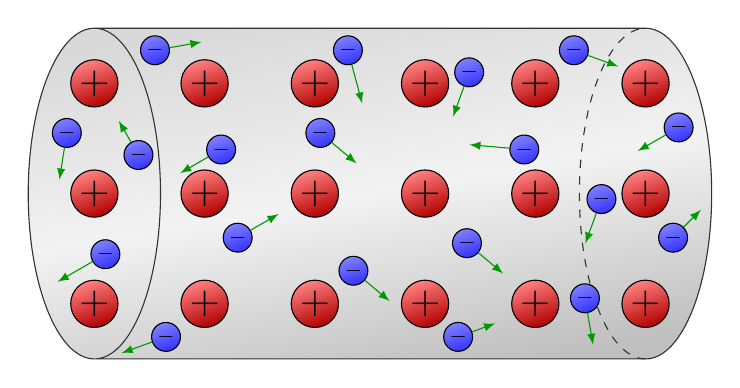
\begin{tikzpicture}
  \def\R{0.3}
  \def\a{1.4}
  \def\Nx{6}
  \def\Ny{3}
  \def\L{\a*(\Nx-1)}
  \def\Rx{0.2*\a*\Ny}
  \def\Ry{1.0*\a*\Ny/2}
  \def\electron#1#2#3{
    \node[charge-,draw=black,circle,fill,inner sep=1,scale=0.8] (e) at (#1*\a,#2*\a) {$-$};
    \draw[->,green!60!black] (e) --++ (#3);
  }
  
  \fill[metal] (0,{-\Ry}) arc (270:90:{\Rx} and {\Ry}) --++ ({\L},0) arc (90:-90:{\Rx} and {\Ry});
  \draw[black!80] (0,{-\Ry}) arc (270:90:{\Rx} and {\Ry});
  \draw[black!80,dashed] ({\L},{-\Ry}) arc (270:90:{\Rx} and {\Ry});
  
  % IONS
  \foreach \j [evaluate={\y=\a*(\j-\Ny/2-0.5);}] in {1,...,\Ny}{
    \foreach \i in {1,...,\Nx}{ %[evaluate={\x=\j*\a;}]
      \draw[charge+] ({(\i-1)*\a},\y) circle (\R) node[scale=1.4] {$+$};
    }
  }
  
  %%%%%%%%%%%%%%%%%%%%%%%%%%%%%%%%% 0
  \electron{-0.25}{ 0.55}{ -99:0.6}
  %%%%%%%%%%%%%%%%%%%%%%%%%%%%%%%%% 1
  \electron{ 0.10}{-0.55}{ 210:0.7}
  \electron{ 0.40}{ 0.35}{ 120:0.5}
  \electron{ 0.55}{ 1.30}{  10:0.6}
  %%%%%%%%%%%%%%%%%%%%%%%%%%%%%%%%% 2
  \electron{ 0.65}{-1.30}{-160:0.6}
  \electron{ 1.30}{-0.40}{  30:0.6}
  \electron{ 1.15}{ 0.40}{ 210:0.6}
  %%%%%%%%%%%%%%%%%%%%%%%%%%%%%%%%% 3
  \electron{ 2.35}{-0.70}{ -40:0.6}
  \electron{ 2.05}{ 0.55}{ -40:0.6}
  \electron{ 2.30}{ 1.30}{ -75:0.7}
  %%%%%%%%%%%%%%%%%%%%%%%%%%%%%%%%% 4
  \electron{ 3.30}{-1.30}{  20:0.5}
  \electron{ 3.40}{ 1.10}{-110:0.6}
  %%%%%%%%%%%%%%%%%%%%%%%%%%%%%%%%% 5
  \electron{ 3.38}{-0.45}{ -40:0.6}
  \electron{ 3.90}{ 0.40}{ 175:0.7}
  \electron{ 4.35}{ 1.30}{ -20:0.6}
  %%%%%%%%%%%%%%%%%%%%%%%%%%%%%%%%% 6
  \electron{ 4.45}{-0.95}{ -80:0.6}
  \electron{ 5.25}{-0.40}{  45:0.5}
  \electron{ 4.60}{-0.05}{-110:0.6}
  \electron{ 5.30}{ 0.60}{-150:0.6}
  %%%%%%%%%%%%%%%%%%%%%%%%%%%%%%%%%
  
  \draw[black!80] (0,{-\Ry}) arc (-90:90:{\Rx} and {\Ry}) --++ ({\L},0) arc (90:-90:{\Rx} and {\Ry}) -- cycle;
  
\end{tikzpicture}


% CONDUCTION MODEL
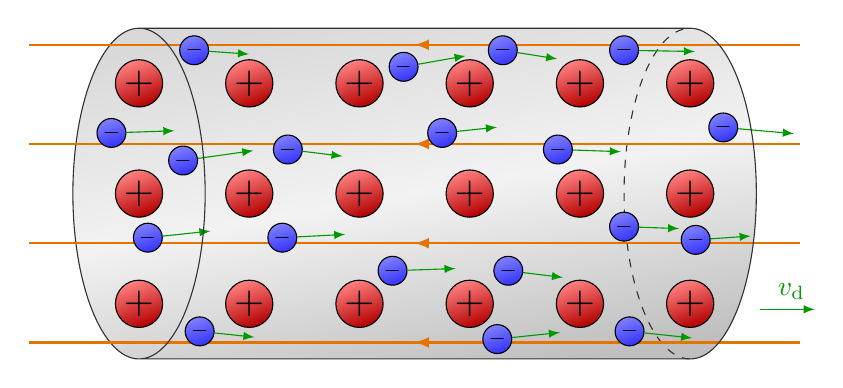
\begin{tikzpicture}
  \def\R{0.3}
  \def\a{1.4}
  \def\Nx{6}
  \def\Ny{3}
  \def\L{\a*(\Nx-1)}
  \def\Rx{0.2*\a*\Ny}
  \def\Ry{1.0*\a*\Ny/2}
  \def\electron#1#2#3{
    \node[charge-,draw=black,circle,fill,inner sep=1,scale=0.8] (e) at (#1*\a,#2*\a) {$-$};
    \draw[->,green!60!black] (e) --++ (#3);
  }
  
  \fill[metal] (0,{-\Ry}) arc (270:90:{\Rx} and {\Ry}) --++ ({\L},0) arc (90:-90:{\Rx} and {\Ry});
  \draw[black!80] (0,{-\Ry}) arc (270:90:{\Rx} and {\Ry});
  \draw[black!80,dashed] ({\L},{-\Ry}) arc (270:90:{\Rx} and {\Ry});
  
  % IONS
  \foreach \j [evaluate={\y=\a*(\j-\Ny/2-0.5);}] in {1,...,\Ny}{
    \foreach \i in {1,...,\Nx}{ %[evaluate={\x=\j*\a;}]
      \draw[charge+] ({(\i-1)*\a},\y) circle (\R) node[scale=1.4] {$+$};
    }
  }
  
  % ELECTRIC FIELD
  \foreach \j [evaluate={\y=0.9*\a*(\j-\Ny/2);}] in {0,...,\Ny}{
    \draw[EField] ({\L+\a},\y) -- (-\a,\y);
  }
  
  %%%%%%%%%%%%%%%%%%%%%%%%%%%%%%%%% 0
  \electron{-0.25}{ 0.55}{  2:0.8}
  %%%%%%%%%%%%%%%%%%%%%%%%%%%%%%%%% 1
  \electron{ 0.08}{-0.40}{  6:0.8}
  \electron{ 0.40}{ 0.30}{  8:0.9}
  \electron{ 0.50}{ 1.30}{ -4:0.7}
  %%%%%%%%%%%%%%%%%%%%%%%%%%%%%%%%% 2
  \electron{ 0.55}{-1.25}{ -6:0.7}
  \electron{ 1.30}{-0.40}{  3:0.8}
  \electron{ 1.35}{ 0.40}{ -7:0.7}
  %%%%%%%%%%%%%%%%%%%%%%%%%%%%%%%%% 3
  \electron{ 2.30}{-0.70}{  2:0.8}
  \electron{ 2.75}{ 0.55}{  6:0.7}
  \electron{ 2.40}{ 1.15}{ 10:0.8}
  %%%%%%%%%%%%%%%%%%%%%%%%%%%%%%%%% 4
  \electron{ 3.25}{-1.32}{  6:0.8}
  \electron{ 3.30}{ 1.30}{ -9:0.7}
  %%%%%%%%%%%%%%%%%%%%%%%%%%%%%%%%% 5
  \electron{ 3.35}{-0.70}{ -7:0.7}
  \electron{ 3.80}{ 0.40}{ -2:0.8}
  \electron{ 4.40}{ 1.30}{ -1:0.9}
  %%%%%%%%%%%%%%%%%%%%%%%%%%%%%%%%% 6
  \electron{ 4.45}{-1.25}{ -6:0.8}
  \electron{ 5.05}{-0.42}{  4:0.7}
  \electron{ 4.40}{-0.30}{ -2:0.7}
  \electron{ 5.30}{ 0.60}{ -5:0.9}
  %%%%%%%%%%%%%%%%%%%%%%%%%%%%%%%%%
  
  \draw[->,green!60!black] ({\L+1.05*\Rx},-0.7*\Ry) --++ (0.7,0) node[above left] {$v_\mathrm{d}$};
  \draw[black!80] (0,{-\Ry}) arc (-90:90:{\Rx} and {\Ry}) --++ ({\L},0) arc (90:-90:{\Rx} and {\Ry}) -- cycle;
  
\end{tikzpicture}


% CONDUCTION MODEL
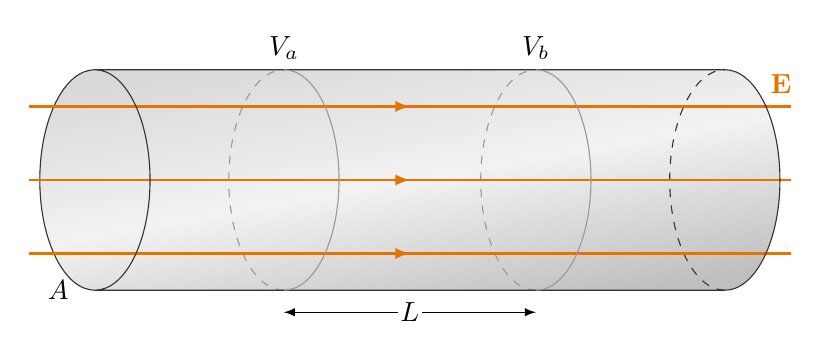
\begin{tikzpicture}
  \def\NE{3}
  \def\L{8}
  \def\a{0.3*\L}
  \def\b{0.7*\L}
  \def\Rx{0.7}
  \def\Ry{1.4}
  
  \fill[metal] (0,-\Ry) arc (270:90:{\Rx} and {\Ry}) --++ ({\L},0) arc (90:-90:{\Rx} and {\Ry});
  \draw[black!80] (0,-\Ry) arc (270:90:{\Rx} and {\Ry});
  \draw[black!80,dashed] (\L,-\Ry) arc (270:90:{\Rx} and {\Ry});
  \draw[black!40,dashed] (\a,-\Ry) arc (270:90:{\Rx} and {\Ry});
  \draw[black!40,dashed] (\b,-\Ry) arc (270:90:{\Rx} and {\Ry});
  
  % ELECTRIC FIELD
  \foreach \j [evaluate={\y=-\Ry+(\j-0.5)*2*\Ry/\NE;}] in {1,...,\NE}{
    \draw[EField] (-1.2*\Rx,\y) -- (\L+1.2*\Rx,\y);
  }
  
  \draw[black!80] (0,-\Ry) arc (-90:90:{\Rx} and {\Ry}) --++ (\L,0) arc (90:-90:{\Rx} and {\Ry}) -- cycle;
  \draw[black!40] (\a,-\Ry) arc (-90:90:{\Rx} and {\Ry});
  \draw[black!40] (\b,-\Ry) arc (-90:90:{\Rx} and {\Ry});
  \draw[<->] (\a,-1.2*\Ry) -- (\b,-1.2*\Ry) node[midway,fill=white,inner sep=1] {$L$};
  \node[above] at (\a,\Ry) {$V_a$};
  \node[above] at (\b,\Ry) {$V_b$};
  \node[left=6] at (0,-\Ry) {$A$};
  \node[below=5,right=13,Ecol] at (\L,\Ry) {$\vb{E}$};
  
\end{tikzpicture}


\end{document}